\section{Objectives}
Cover both Lab 4.A differential voltage amplifiers and Lab 4.B differential current amplifiers from \textit{AIC Lab.pdf}, PDF pages 41--47. The model library is supplied separately by the user. The 1.0 V supply is a teaching adaptation, not a certification of the model voltage rating. Numerical plots for the handout's original 3.3 V process are not used directly as pass thresholds. The circuits are rebuilt from the handout topology; the earlier code is used only to review dimensions and omissions.

\section{Specification Mapping}
S denotes actual simulation and D derivation/discussion. D01 identifies the filename prefix; case numbering starts at C0.
\small\begin{longtable}{p{.46\linewidth}p{.30\linewidth}p{.15\linewidth}}\toprule
Requirement and PDF pages & Deck / check & Status \\ \midrule\endhead
Three differential voltage amplifiers (41--42) & D01--03 & S+D \\
ICMR and device saturation checks (42) & D04; 21 points & S+D \\
Gain, GB, CMRR and PSRR (43--44) & D01--03; AC families & S+D \\
Equal-W/L scaling and cascode comparison (44) & D01/C4--6; D02--03 & S+D \\
Three current amplifiers and 1 kOhm load (45--47) & D05 & S+D \\
100/1000/10000 um widths and Rin/Rout (46--47) & D05/C1--12 & S+D \\
PMOS source dimensions and tradeoffs (47) & D05/C13 & S+D \\
\bottomrule\end{longtable}\normalsize


\section{Circuit and Design Derivation}
\[
 A_d\simeq\frac{g_m}{g_{ds,n}+g_{ds,p}},\qquad
 f_u\simeq\frac{g_m}{2\pi C_L},\qquad
 \mathrm{CMRR}_{dB}=20\log_{10}\left|\frac{A_d}{A_{cm}}\right|.
 \]
 \[
 \mathrm{PSRR}_{\pm,dB}=20\log_{10}\left|\frac{A_d}{A_{supply,\pm}}\right|,
 \quad R_{in}\simeq1/g_{m,in},\quad A_i\simeq\frac{(W/L)_{out}}{(W/L)_{in}}.
 \]Voltage amplifiers use $C_L=10$ pF. The basic reference is 50 $\mu$A; cascode baseline comparisons explicitly use 0.5 $\mu$A to retain 1 V headroom, with 50 $\mu$A cases also retained. M1/M2 use $425/0.3\,\mu$m, PMOS loads $1350/0.3\,\mu$m, and reference/tail devices $85/0.3$ and $870/0.3\,\mu$m. D01/C4,C5 scale both W and L of input/load devices by 3,5 without changing the tail mirror. Full-cascode extra NMOS gates are held at 0.6 V.

The current amplifier deck contains simple (s), cascode (c) and differential (d) versions. Reference NMOS width is 50 $\mu$m; output width is 100/1000/10000 $\mu$m; $L=0.3\,\mu$m. A real 1 k$\Omega$ load is grounded. C0 retains matched source/sink currents, potentially driving the output near ground and outside its operating region. C1--3 explicitly add nominal 0.5 mA PMOS bias to place the load near 0.5 V. C7--9 change both lower cascode widths. C13 doubles s/c PMOS source widths; the first d PMOS also changes but its other two remain ratio-defined, making d an additional imbalance counterexample, not a matched comparison.

\section{Simulation Setup}
Runs use PrimeSim HSPICE S-2021.09 win64, a baseline temperature of 27 $^\circ$C, \texttt{runlvl=5}, \texttt{accurate}, and \texttt{.op/.print/.measure} outputs. Every \texttt{.alter} resets all baseline parameters and temperature to prevent state from carrying into the next case. Actual runs completed without an error or failed measurement. Suppressed model warnings remain, so a warning-free run is not claimed. Public netlists contain no model paths. This comment marks the model setup required locally before execution; the model and its configuration remain local:
\begin{verbatim}
* MODEL_SETUP_REQUIRED
\end{verbatim}
CSV files and numerical summaries are in the lab's \texttt{results/} directory. Every figure is redrawn from actual printed data, not a waveform-viewer screenshot. \texttt{manifest.json} supplies specification mapping and case definitions.Five decks contain 52 cases. AC sweeps 1 Hz--10 GHz with 60 points/decade. Differential voltage is $+0.5/-0.5$ V, hence 1 V total; common mode drives both inputs with 1 V. Supply injection holds ideal inputs relative to global ground. Differential current uses $+0.5/-0.5$ A. ICMR sweeps 0--1 V in 50 mV steps with device $V_{DS}$ and $V_{DSAT}$ stored at every point. Rout cases disable input AC and inject 1 A, using a huge series load inductor to retain DC bias while removing the 1 k$\Omega$ AC load. This is a measurement fixture, not a realizable inductor.

\section{Results and Specification Checks}
\begin{center}\small\begin{tabular}{lrrrr}\toprule
Case & $A_d$ (dB) & $f_{3dB}$ (kHz) & $f_u$ (MHz) & $V_o$ (V) \\ \midrule
D01/C0 & 39.60 & 620.351 & 59.217 & 0.7002 \\
D01/C4 & 45.44 & 197.286 & 32.930 & 0.6921 \\
D01/C5 & 46.53 & 125.985 & 22.035 & 0.6907 \\
D01/C6 & 32.58 & 21.771 & 0.874 & 0.8885 \\
D02/C0 & 46.82 & 4.259 & 0.750 & 0.7530 \\
D02/C4 & 41.17 & 608.640 & 55.649 & 0.3427 \\
D03/C0 & 68.26 & 0.349 & 0.730 & 0.7523 \\
D03/C4 & 54.58 & 125.026 & 54.085 & 0.3428 \\
\bottomrule\end{tabular}\end{center}
\begin{center}\small\begin{tabular}{lrrr}\toprule
Topology & CMRR (dB) & PSRR+ (dB) & PSRR- (dB) \\ \midrule
Basic & 81.18 & 39.60 & 81.14 \\
Load cascode & 87.03 & 46.82 & 86.73 \\
Full cascode & 130.18 & 68.26 & 108.07 \\
\bottomrule\end{tabular}\end{center}

\begin{figure}[htbp]\centering
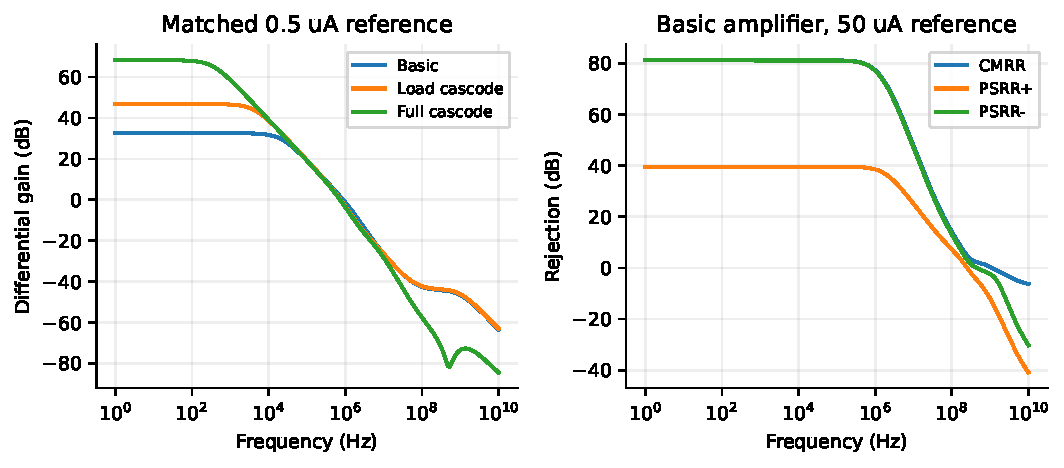
\includegraphics[width=\linewidth]{figures/voltage_amplifiers.pdf}
\caption{Left: three topologies at matched 0.5 microamp reference. Right: rejection for the 50 microamp basic amplifier; the panel biases differ.}
\end{figure}
For the common 0.5 $\mu$A scan, contiguous sampled intervals with every device satisfying $|V_{DS}|\ge|V_{DSAT}|$ are 0.20--1.00 V (basic), 0.20--0.95 V (load cascode) and 0.20--0.55 V (full cascode). Endpoint resolution is 50 mV, and the basic upper bound reaches the sweep limit. This criterion does not establish strong inversion or constant transconductance.
\begin{center}\small\begin{tabular}{lrrrrr}\toprule
Case/Type & $|A_i|$ & $R_{in}$ (k$\Omega$) & $R_o$ (k$\Omega$) & $f_{3dB}$ (MHz) & $V_o$ (V) \\ \midrule
C0/s & 0.501 & 4.061 & -- & 112.679 & 0.013 \\
C0/c & 0.503 & 9.127 & -- & 340.870 & 0.014 \\
C0/d & 0.731 & 7.958 & -- & 49.273 & 0.013 \\
C1/s & 1.916 & 4.061 & 15.814 & 0.778 & 0.512 \\
C1/c & 1.864 & 9.133 & 16.392 & 0.792 & 0.514 \\
C1/d & 2.797 & 7.958 & 15.814 & 0.794 & 0.512 \\
C2/s & 18.415 & 4.059 & 9.522 & 0.459 & 0.502 \\
C2/c & 18.271 & 9.134 & 12.146 & 0.443 & 0.515 \\
C2/d & 158.918 & 36.990 & 9.525 & 0.440 & 0.502 \\
C3/s & 127.907 & 4.009 & 1.744 & 0.025 & 0.436 \\
C3/c & 150.941 & 9.135 & 3.316 & 0.022 & 0.534 \\
C3/d & 1511.730 & 121.390 & 0.271 & 0.022 & 0.082 \\
C13/s & 0.751 & 2.114 & -- & 0.302 & 0.921 \\
C13/c & 0.678 & 4.770 & -- & 0.319 & 0.923 \\
C13/d & 0.007 & 4.192 & -- & 290.717 & 0.533 \\
\bottomrule\end{tabular}\end{center}
\begin{center}\small\begin{tabular}{lrrrr}\toprule
Lower width ($\mu$m) & $|A_i|$ & $R_{in}$ (k$\Omega$) & $R_o$ (k$\Omega$) & $f_{3dB}$ (MHz) \\ \midrule
100 & 0.935 & 8.949 & 16.337 & 0.810 \\
1000 & 0.936 & 8.528 & 16.337 & 0.793 \\
10000 & 0.895 & 7.674 & 16.325 & 0.533 \\
\bottomrule\end{tabular}\end{center}

\begin{figure}[htbp]\centering
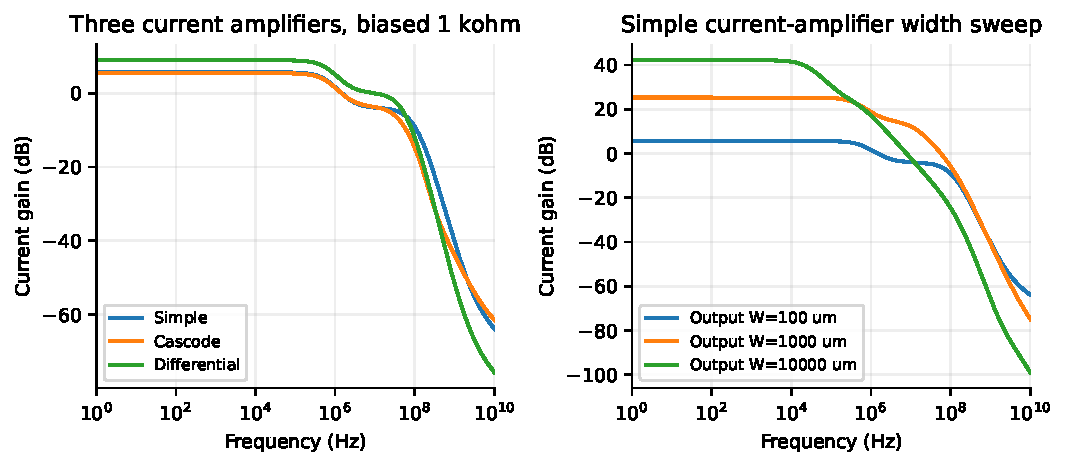
\includegraphics[width=\linewidth]{figures/current_amplifiers.pdf}
\caption{Left: the three current amplifiers in C1. Right: simple-amplifier output-width sweep including actual bias and loading.}
\end{figure}
The s/c/d labels denote simple/cascode/differential current amplifiers. Failed operating regions in C0, imbalance in C13 and actual output voltages remain in the results. Values disagreeing with square-law predictions are retained. A dash means Rout was not measured independently for that case. Full CSV data preserve the frequency dependence.

\section{Discussion}
Compared with a single-ended CS, differential inputs reject common disturbances and support negative feedback, but require more devices, bias current, matching and common-mode headroom. Increasing device length at equal W/L reduces output conductance: basic gain rises from 39.60 dB to 45.44/46.53 dB while bandwidth decreases. Cascoding raises output impedance and gain at the cost of headroom; full cascode has the narrowest ICMR at matched low current. Rejection assumes nominal matching, without mismatch or silicon guarantees.

The simple current mirror needs less headroom and capacitance. Cascode internal nodes and body effect can raise input impedance while reducing loaded current gain. Larger output W and bias increase ideal mirror ratio but also capacitance and output conductance, so Rin, Rout and GB do not improve together. PMOS sizing changes DC balance: C13 approaches the upper rail and must be interpreted with its bias. The differential current topology accepts two inputs but accumulates errors and capacitance across mirror stages. The text, width tables and plot names on pages 46--47 are not fully consistent; the explicitly listed devices and cases define this report, without imposing the old numbers.

\section{Conclusion}
Every topology, measurement and discussion in Lab 4.A/B is represented. Actual results show gain, rejection and operating-region tradeoffs, including failed bias cases. Original-process numbers and manufacturing validation are not claimed.

